\section{Haskell}

\begin{frame}[fragile]\frametitle{Immutable}

No self-assignment

\begin{verbatim}
let x = 1
    x = x + 1
print x
\end{verbatim}

\end{frame}

\begin{frame}[fragile]\frametitle{Immutable}

Name can be recycled but moved to another (memory) location.

\begin{verbatim}
let x = 1
    x = 2
print x
\end{verbatim}

\end{frame}

\begin{frame}\frametitle{Immutable}

\begin{itemize}
\item
  Immutable is about purity
\item
  Purity is how a programmer designs the code to separate pure and
  effects code
\item
  Purity is what keeps compiler faster, generate optimised code.
\end{itemize}

\end{frame}

\begin{frame}\frametitle{Immutable v.s. Mutables}

\begin{itemize}
\item
  What's good in mutables?

  \begin{itemize}
  \item
    Convenience: in-place modification
  \item
    Speed
  \end{itemize}
\item
  What's bad in mutables?

  \begin{itemize}
  \item
    no problem in ST
  \item
    many problems in MT
  \end{itemize}
\end{itemize}

\end{frame}

\begin{frame}\frametitle{Application pattern}

\begin{itemize}
\item
  Pattern 1:
\end{itemize}

\begin{enumerate}[1.]
\item
  get input from outside
\item
  process
\item
  sent output to outside
\end{enumerate}

\begin{itemize}
\item
  Pattern 2:
\end{itemize}

\begin{enumerate}[1.]
\item
  \ldots{}
\item
  process: interact with outside
\item
  \ldots{}
\end{enumerate}

\end{frame}

\begin{frame}[fragile]\frametitle{Solution}

\begin{itemize}
\item
  The process is a recursive function to transform state

\begin{verbatim}
f :: State -> ... -> State
\end{verbatim}
\end{itemize}

\end{frame}

\begin{frame}\frametitle{Solution}

\begin{itemize}
\item
  Think and Plan:

  \begin{itemize}
  \item
    How often it get changed?
  \item
    What scope does it affected? limited, global
  \item
    What's the requirement, need for speed?
  \end{itemize}
\end{itemize}

\end{frame}

\begin{frame}\frametitle{Haskell's Solution}

\begin{itemize}
\item
  Localized

  \begin{itemize}
  \item
    State Monad
  \item
    ST Monad
  \end{itemize}
\item
  Closed but operate from inside

  \begin{itemize}
  \item
    StateT Monad Transformer
  \end{itemize}
\item
  Open

  \begin{itemize}
  \item
    IORef
  \item
    MVar
  \item
    TVar (STM, not covered)
  \end{itemize}
\end{itemize}

\end{frame}

\section{Problem}

\begin{frame}\frametitle{DNA Sequence Statistics}

\begin{itemize}
\item
  DNA: A, T, G, C
\end{itemize}

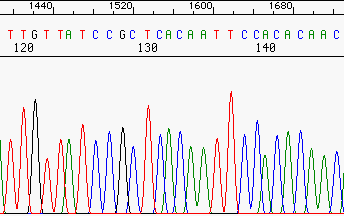
\includegraphics[width=4in]{img/normal3730.png}

\end{frame}

\begin{frame}[fragile]\frametitle{DNA Sequence}

\begin{verbatim}
CCCCTGATCGAATTCCTATTCTAGCCGCTCCTGCCGTTTTGC
GTCTGCGGCGTGTAGCGCGTATCACAGTTCGAGGTGGAATCA
CTGCACAAGGGATTAGTGGGAGATAGTATGGGGCGTGTCGGG
TTTAGTAGTGTCCGTGAAGCGAGCACACACTCTGAACGTATT
GCACATAGTACTTAGCAATCCTTCGCACCCCATGGTGTGGGA
TCGTGAACCGTAGCCGTGGGTAGATCTCTTCGATTGAGCGAA
....
\end{verbatim}

A:XX\%, T:YY\%, G:ZZ\%, C:WW\%

\end{frame}

\begin{frame}[fragile]\frametitle{Python code}

\begin{verbatim}
seq = "ACCCCTGATCGA..."

d = { "A": 0, "C": 0, "G": 0, "T": 0 }

for nuc in seq:
    d[nuc]+=1

print d["A"], d["C"], d["G"], d["T"]
\end{verbatim}

\end{frame}

\begin{frame}[fragile]\frametitle{Haskell}

\begin{verbatim}
type SeqInfo = (Int, Int, Int, Int)
emptySeqInfo = (0,0,0,0)

countSeq :: Char -> SeqInfo -> SeqInfo
countSeq n w@(a,t,g,c) = case n of
    'A' -> (a+1,t,g,c)
    'T' -> (a,t+1,g,c)
    'G' -> (a,t,g+1,c)
    'C' -> (a,t,g,c+1)
    otherwise -> w

countNuc :: String -> SeqInfo
countNuc seq = foldl (flip countSeq) emptySeqInfo seq
\end{verbatim}

\end{frame}

\begin{frame}[fragile]\frametitle{Haskell - 2}

\begin{verbatim}
main :: IO ()
main = do
    seq <- readFile "seq.dna"
    let (cA, cT, cG, cC) = countNuc seq
    putStrLn ("A:" ++ show cA ++ " T:" ++ show cT
          ++ " G:" ++ show cG ++ " C:" ++ show cC)
\end{verbatim}

Classic example of pattern 1

\end{frame}

\begin{frame}[fragile]\frametitle{State Monad}

\begin{itemize}
\item
  State and its relative ST both produce `monolithic' stateful
  computations which may be run as units.
\item
  API: get, put, runState

\begin{verbatim}
State (String, SeqInfo)

countNuc2 :: String -> SeqInfo
countNuc2 seq = (cA, cT, cG, cC)
    where (s, (cA, cT, cG, cC)) = 
             runState (calc seq) emptySeqInfo 
             :: (String, (Int, Int, Int, Int))
          calc (x:xs) = do
            (a,t,g,c) <- get
            put $ countSeq x (a,t,g,c)
            calc xs
          calc [] = return ""
\end{verbatim}
\end{itemize}

\end{frame}

\begin{frame}[fragile]\frametitle{ST Monad}

The mutable state is localized and do not require interaction with the
environment.

\begin{itemize}
\item
  API

  \begin{itemize}
  \item
    runST: start a new memory-effect computation.
  \item
    STRefs: pointers to (local) mutable cells.
  \item
    ST-based arrays

\begin{verbatim}
countNuc2ST :: String -> SeqInfo
countNuc2ST seq = runST $ do
    cseq <- newSTRef emptySeqInfo
    forM_ seq $ (modifySTRef cseq) . countSeq
    readSTRef cseq                                  
\end{verbatim}
  \end{itemize}
\end{itemize}

\end{frame}

\begin{frame}[fragile]\frametitle{StateT Monad Transformer}

\begin{itemize}
\item
  StateT SeqInfo IO ()

\begin{verbatim}
countNuc5 :: String  -> IO SeqInfo  
countNuc5 seq = do
    (_, cseq) <- runStateT (calc seq) emptySeqInfo
    return cseq
    where calc :: String -> StateT SeqInfo IO ()
        calc (x:xs) = do
            w <- get
            put $ countSeq x w
            calc xs
        calc [] = return ()
\end{verbatim}
\end{itemize}

\end{frame}

\begin{frame}[fragile]\frametitle{Interactive with StateT Monad}

\begin{verbatim}
countNuc6 cseq = runStateT calc cseq
    where calc :: StateT SeqInfo IO ()
        calc = do
            n <- io $ hGetChar stdin
            if n == '\n' then return ()
            else do
                w <- get
                let w1 = countSeq n w 
                put w1
                let (cA, cT, cG, cC) = w1
                io $ when (w1 /= w) $
                putStrLn (n : " (A:" ++ show cA ++ " T:"
                    ++ show cT ++ " G:"
                    ++ show cG ++ " C:"
                    ++ show cC ++ ")") 
                calc
        io = liftIO
\end{verbatim}

\end{frame}

\begin{frame}\frametitle{IORef/MVar}

\begin{itemize}
\item
  IORef is not a `computation' to be run -- it is just a box holding a
  simple value which may be used within IO in fairly arbitrary ways.
\item
  IORef and MVar

  \begin{enumerate}[1.]
  \item
    Concurrency: IORef use atomicModifyIORef, MVar uses a more general
    approach.
  \item
    MVar provides empty and fill two states, use for synchronization.
  \end{enumerate}
\end{itemize}

\end{frame}

\begin{frame}[fragile]\frametitle{IORef}

\begin{itemize}
\item
  API: newIORef, modifyIORef.

\begin{verbatim}
modifyIORef :: IORef a -> (a -> a) -> IO ()

countSeqIORef :: Char -> IORef SeqInfo -> IO ()
countSeqIORef n cseq = modifyIORef cseq $ countSeq n 

countNuc3 :: String -> IORef SeqInfo -> IO SeqInfo 
countNuc3 seq cseq = do
    mapM_ (flip countSeqIORef $ cseq) seq
    return =<< readIORef cseq 
\end{verbatim}
\end{itemize}

\end{frame}

\begin{frame}[fragile]\frametitle{MVar}

\begin{itemize}
\item
  API: newMVar, takeMVar, putMVar, modifyMVar

\begin{verbatim}
modifyMVar :: MVar a -> (a -> IO a) -> IO () 

countSeqMVar :: Char -> MVar SeqInfo -> IO ()
countSeqMVar n cseq = takeMVar cseq >>= (putMVar cseq) . (countSeq n)

countNuc4 :: String -> MVar SeqInfo -> IO SeqInfo
countNuc4 seq cseq = do
    mapM_ ((flip countSeqMVar) cseq) seq
    return =<< readMVar cseq
\end{verbatim}
\end{itemize}

\end{frame}

\begin{frame}[fragile]\frametitle{Network server}

\begin{verbatim}
countSeqHandler :: MVar SeqInfo -> HandlerFunc
countSeqHandler mcseq addr msg = do
    (cA, cT, cG, cC) <- readMVar mcseq 
    mapM_ ((flip countSeqMVar) mcseq) msg 

main :: IO ()
main = do
    mcseq <- newMVar emptySeqInfo
    serveStub "11111" $ countSeqHandler mcseq 
\end{verbatim}

\end{frame}

\section{Summary}

\begin{frame}\frametitle{Summary}

\begin{itemize}
\item
  State Monad and ST Monad: State provides a cleanest solution.
\item
  StateT Monad Transformer: Interactive, storing global state in game
\item
  IORef/MVar/TVar(STM, not covered): Mutable state which may be passed
  around and interacted with in controlled ways by IO code, MVar
  (faster), STM/TVar(slower)
\end{itemize}

\end{frame}

\begin{frame}\frametitle{Benchmark: no Option}

\begin{itemize}
\item
  CountSeq/foldl'

  \begin{itemize}
  \item
    mean: 8.367447 ms, lb 8.218304 ms, ub 8.597044 ms, ci 0.950
  \end{itemize}
\item
  CountSeq/State Monad

  \begin{itemize}
  \item
    mean: 29.00443 ns, lb 28.40861 ns, ub 30.51695 ns, ci 0.950
  \end{itemize}
\item
  CountSeq/ST Monad

  \begin{itemize}
  \item
    mean: 16.29765 ms, lb 16.01618 ms, ub 16.78243 ms, ci 0.950
  \end{itemize}
\item
  CountSeq/IORef

  \begin{itemize}
  \item
    mean: 14.39716 ms, lb 13.95155 ms, ub 15.11095 ms, ci 0.950
  \end{itemize}
\item
  CountSeq/MVar

  \begin{itemize}
  \item
    mean: 18.46335 ms, lb 18.09122 ms, ub 18.99158 ms, ci 0.950
  \end{itemize}
\item
  CountSeq/StateT

  \begin{itemize}
  \item
    mean: 22.35278 ms, lb 21.90441 ms, ub 23.02252 ms, ci 0.950
  \end{itemize}
\end{itemize}

\end{frame}

\begin{frame}\frametitle{Benchmark: -O}

\begin{itemize}
\item
  CountSeq/foldl'

  \begin{itemize}
  \item
    mean: 738.3003 us, lb 715.5623 us, ub 763.9446 us, ci 0.950
  \end{itemize}
\item
  CountSeq/State Monad

  \begin{itemize}
  \item
    mean: 24.28070 ns, lb 23.67202 ns, ub 24.98461 ns, ci 0.950
  \end{itemize}
\item
  CountSeq/ST Monad

  \begin{itemize}
  \item
    mean: 13.34422 ms, lb 12.95808 ms, ub 13.84491 ms, ci 0.950
  \end{itemize}
\item
  CountSeq/IORef

  \begin{itemize}
  \item
    mean: 10.47555 ms, lb 10.22925 ms, ub 10.75831 ms, ci 0.950
  \end{itemize}
\item
  CountSeq/MVar

  \begin{itemize}
  \item
    mean: 10.67125 ms, lb 10.37612 ms, ub 11.02434 ms, ci 0.950
  \end{itemize}
\item
  CountSeq/StateT

  \begin{itemize}
  \item
    mean: 10.57837 ms, lb 10.28747 ms, ub 10.90067 ms, ci 0.950
  \end{itemize}
\end{itemize}

\end{frame}

\begin{frame}\frametitle{Benchmark: -O3}

\begin{itemize}
\item
  Build with -O3
\item
  CountSeq/foldl'

  \begin{itemize}
  \item
    mean: 499.2094 us, lb 487.7534 us, ub 512.6872 us, ci 0.950
  \end{itemize}
\item
  CountSeq/State Monad

  \begin{itemize}
  \item
    mean: 26.12395 ns, lb 25.36894 ns, ub 26.92742 ns, ci 0.950
  \end{itemize}
\item
  CountSeq/ST Monad

  \begin{itemize}
  \item
    mean: 10.44361 ms, lb 10.16934 ms, ub 10.74252 ms, ci 0.950
  \end{itemize}
\item
  CountSeq/IORef

  \begin{itemize}
  \item
    mean: 10.73348 ms, lb 10.44679 ms, ub 11.05740 ms, ci 0.950
  \end{itemize}
\item
  CountSeq/MVar

  \begin{itemize}
  \item
    mean: 11.03261 ms, lb 10.72550 ms, ub 11.37463 ms, ci 0.950
  \end{itemize}
\item
  CountSeq/StateT

  \begin{itemize}
  \item
    mean: 10.63487 ms, lb 10.37687 ms, ub 10.92361 ms, ci 0.950
  \end{itemize}
\end{itemize}

\end{frame}
